\documentclass[12pt, a4paper]{article}
\usepackage[utf8]{inputenc}
\usepackage{amsmath, amssymb, amsthm}
\usepackage[margin=2.5cm]{geometry}
\usepackage{enumitem}
\usepackage[utf8]{inputenc}
\usepackage[T1]{fontenc}
\usepackage{amsmath, amssymb, amsthm}
\usepackage{mathtools}
\usepackage{geometry}
\usepackage{setspace}
\usepackage{booktabs}
\usepackage{array}
\usepackage{bm}
\usepackage{multirow}
\usepackage{caption}
\usepackage{graphicx}
\usepackage{tikz}
\usetikzlibrary{arrows.meta, positioning, calc}
\usepackage{hyperref}
\usepackage[round]{natbib}
\usepackage{xcolor}
\usepackage{longtable}
\usepackage{float}
\usepackage{tcolorbox}
\newcolumntype{P}[1]{>{\raggedright\arraybackslash}p{#1}}
\usepackage{pdflscape}
\usepackage{caption}


\geometry{margin=2.5cm}

\newtheorem{assumption}{Assumption}
\newtheorem{proposition}{Proposition}
\newtheorem{corollary}{Corollary}
\newtheorem{lemma}{Lemma}
\newtheorem{definition}{Definition}
\newtheorem{remark}{Remark}


\begin{document}


\begin{center}
{\large \textsc{University of Basel}} \\
{\textsc{Faculty of Business and Economics}} \\[2cm]
{\LARGE \textbf{Research Proposal}} \\[1.5cm]
Aulis Pesenti \\
PhD Candidate \\
\today
\end{center}

%Am Ende noch ergänzen
\noindent As the first project has progressed substantially beyond the proposal stage, this document serves as a description of the research design and the work completed to date rather than a prospective outline. It is supplemented by preliminary results and concludes with a discussion of the remaining steps and open methodological questions. The accompanying first draft of the paper, referenced throughout, as well as the data description can be found on \textbf{\href{https://github.com/pesentiA/Pandemic-Trilemma}{GitHub}}. The proposed second project can be found from page~\pageref{sec:paper2} onward.

\section{Pandemic Trilemma}


\subsection{The Research Question}


A government confronting a pandemic faces three simultaneous main objectives: protecting public health by minimizing excess mortality, preserving economic stability by minimizing the deviation of output from its potential, and maintaining fiscal sustainability by not destabilizing the level of public debt. Yet while the pandemic struck virtually every economy on the globe, the outcomes across these three dimensions diverged substantially between comparable countries as seen in Figure~\ref{fig:outcomes}.


\begin{figure}[H]
    \centering
    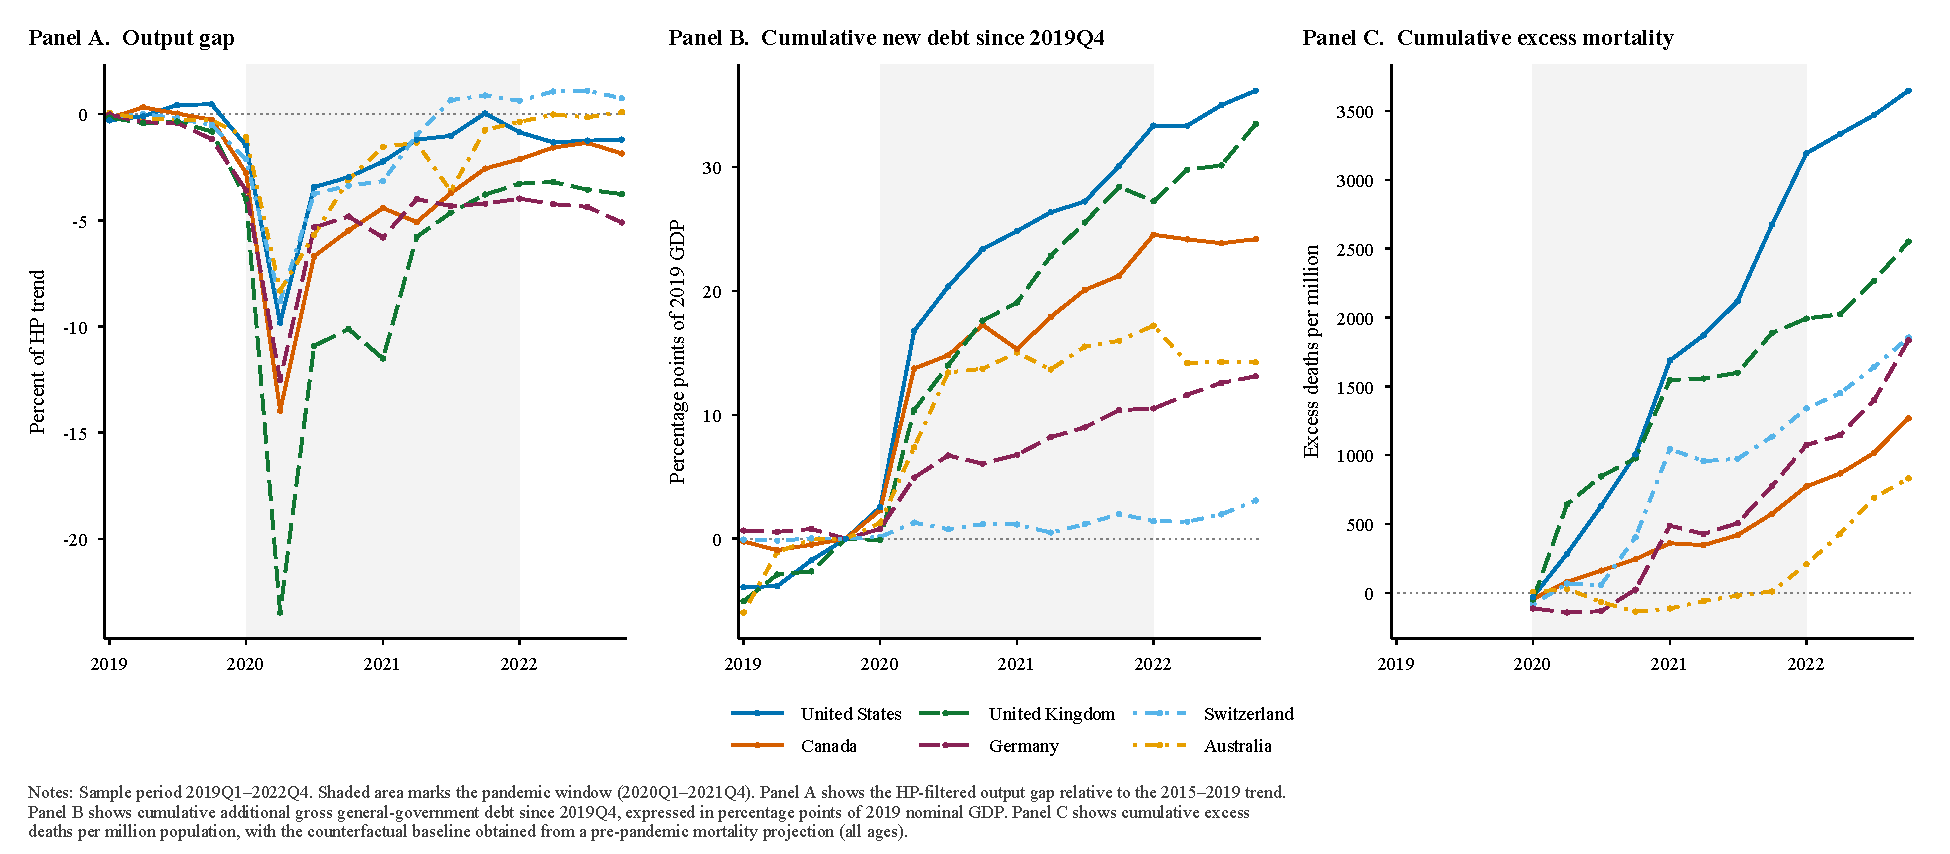
\includegraphics[width=\textwidth]{outcomes_y_cumdebt_excess_aer.pdf}
    \caption{Heterogeneous Outcomes across Dimensions, Selected OECD Countries}
    \label{fig:outcomes}
\end{figure}


\noindent Understanding the source of this divergence requires first an understanding of what distinguishes a pandemic from other macroeconomic crises--- and therefore the structural properties of the environment in which governments were forced to act. The pandemic environment is defined by four structural properties. First, viral prevalence of a deadly pathogen, once introduced exogenously, grows endogenously through human contact. In the absence of a vaccine, suppression is the only available containment instrument, and because it operates through contact reduction, it simultaneously restricts economic activity---establishing the second property: containment is inherently contractionary. Third, containment damages the economy through two distinct channels: it directly reduces the level of output by restricting economic activity and suppressing expenditure, and it erodes the economy's capacity to recover through firm failures, dissolution of employment relationships, and disruption of supply chains. These two channels require fundamentally different fiscal instruments. Demand injection (DI: direct transfers, tax reductions) addresses the level channel through the standard Keynesian multiplier, while capacity preservation (CP: wage subsidies, loans, and guarantees) addresses the persistence channel by preventing the structural destruction that would otherwise prolong the contraction. Both instruments stabilize output but at the cost of public debt accumulation, and their fiscal cost per unit of stabilization differs not only in magnitude but also in its dependence on the state of the economy. Fourth, even in the absence of any discretionary fiscal response, the output contraction itself erodes the fiscal position through falling tax revenues and rising mandatory transfer payments. Fiscal abstinence is therefore not a feasible strategy. 

These four properties jointly impose an inescapable constraint: every policy response to one dimension of the crisis worsens at least one other dimension, and inaction worsens the fiscal dimension regardless. The three objectives are therefore mutually incompatible under the structural architecture of the pandemic environment, forming a \textit{trilemma} in the sense of the Mundell--Fleming impossible trinity \citep{mundell1963}: no feasible policy of a benevolent social planner can simultaneously achieve all three goals, regardless of the resources deployed. This impossibility holds as long as no effective vaccine is available---the condition that defined the period from Q1\,2020 through approximately Q4\,2021, after which widespread vaccination dissolved the binding constraint between containment and output. Section~2 of the attached draft formalizes this result and establishes, through a systematic diagnostic applied to alternative crisis types, that the pandemic is the only macroeconomic crisis in which all four constitutive properties operate simultaneously within a tractable planning horizon.


%%Plot evtl. dazwischen machen evtl. sonst einen zu grossen block
Given this structure, the planner's decision is not whether to intervene but how to compose the intervention. The containment response was largely synchronized across countries: while stringency, measures with an index, varied substantially over the course of the pandemic within each country, the average intensity across the main pandemic years was remarkably similar, ranging only 39 to 48 across six major OECD economies (Panel~A of Figure~\ref{fig:composition2}). The fiscal response, by contrast, diverged substantially in both size and composition (Panel~B): cumulative discretionary spending ranged from 12 to 30 percentage points of 2019 GDP, and the share allocated to demand injection varied from under 10\% to nearly 50\%. Countries facing near-identical containment trajectories chose fundamentally different fiscal strategies---and the composition of these strategies matters as there are two distinct channels to address. Demand injection addresses the level of output and risks being ineffective when the expenditure margin is physically constrained, while capacity preservation addresses the persistence of the shock by preventing structural destruction, but generates no immediate output recovery---the preserved capacity materializes only once containment is lifted. The optimal fiscal response therefore depends not only on its aggregate size but critically on its composition, and because the severity of the supply constraint varies with containment intensity, this composition must adjust dynamically over the course of the pandemic.

\begin{figure}[H]
    \centering
    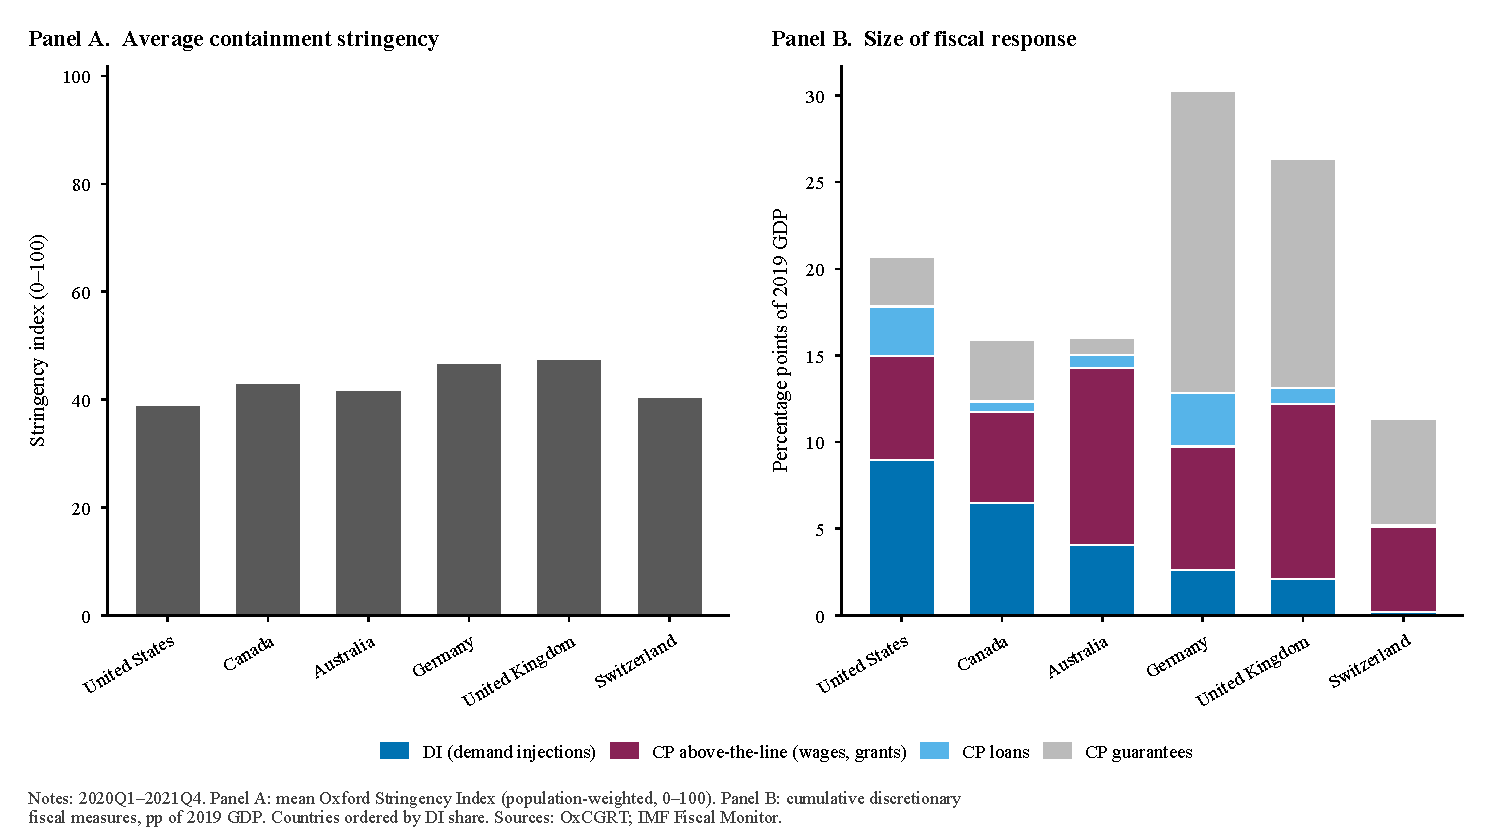
\includegraphics[width=0.7\textwidth]{stringency_vs_fiscal_aer_v2.pdf}
    \caption{Fiscal Response Composition and Size, Selected OECD Countries}
    \label{fig:composition2}
\end{figure}


\noindent The research question therefore is: \textit{What is the optimal composition of fiscal support between capacity preservation and demand injection over the course of a pandemic, given the containment trajectory and epidemiological state faced by each country, and what are the costs—in foregone output stabilization and excess debt—of deviating from this optimum?}

\medskip
\noindent This question has direct policy consequences beyond the historical episode. OECD government debt increased by approximately 15 percentage points of GDP between 2019 and 2021 
\citep{OECD2022borrowing}, with individual countries ranging from near-zero accumulation to over 30 percentage points. Countries that achieved comparable health and economic outcomes at lower 
fiscal cost entered subsequent shocks in a structurally stronger position. Understanding which strategies achieved this, and why, informs three concrete policy margins for future crises: the 
composition of stimulus packages under supply-constrained conditions, the choice between direct expenditure and contingent liabilities in preserving productive capacity, and the 
intertemporal trade-off between output stabilization and fiscal sustainability. %Individual structural parameters might also carry informational value for a broader class of macroeconomic crises: the persistence coefficient $\eta_p$ identifies when capacity-preserving instruments prevent structural destruction in deep recessions, and the heterogeneous fiscal cost across instruments---in particular the near-zero realized cost of credit guarantees---informs the design of contingent fiscal policy wherever governments weigh direct expenditure against contingent liabilities.

%PREDICTIONS NACH DEM MODELL

\subsubsection{Current State of the Literature}
A large literature has studied the optimal policy response to pandemics, but the overwhelming focus has been on containment intensity and its economic consequences. On the macro-modeling side, \citet{Atkeson2020} establishes the baseline susceptible-infected-removed model (SIR) in a macro framework; \citet{alvarez2020} solve for the optimal lockdown trajectory trading off fatalities against output costs; \citet{eichenbaum2021macro} endogenize the behavioral recession by embedding SIR dynamics into a macroeconomic equilibrium; \citet{acemoglu2021} extend the epidemiological framework to age-targeted containment; and \citet{Jones2021} study the endogenous interaction between infection risk and labor supply. On the empirical side, a substantial body of work estimates the effect of non-pharmaceutical interventions on economic activity across countries \citep{Ashraf2022, Konig2020, Cross2020, Gordon2021}, documenting the contractionary impact of containment but treating the fiscal response as given or absent. \citet{KaplanMollViolante2020} come closest to the full trilemma by integrating SIR dynamics into a heterogeneous-agent model with both lockdown and fiscal transfers, but fiscal policy enters as undifferentiated lump-sum transfers and government debt as a residual accounting identity rather than as an optimization target---leaving the compositional and intertemporal fiscal margins outside the optimization problem.

A second strand moves beyond containment and examines the effectiveness of fiscal responses to COVID-19 directly. A large body of country-specific work documents the design and implementation of individual national fiscal packages, providing rich qualitative evidence but no cross-country framework for assessing compositional optimality. Among the quantitative contributions, \citet{chetty2020} use real-time private-sector data to document that U.S.\ direct transfers had limited spending effects during containment; \citet{Autor2022} estimate the employment effects of the Paycheck Protection Program; \citet{Pappa2022} analyze the effectiveness of on-budget fiscal measures on economic growth in 12 EU countries; \citet{fariaecastro2021} shows in a nonlinear DSGE model calibrated to the U.S.\ that the pandemic shock alters the ranking of fiscal policy multipliers, with liquidity assistance dominating transfers for employment stabilization; and \citet{deb2021} provide the most comprehensive cross-country evidence, finding that emergency-lifeline instruments outperform income-support measures during strict containment while the ranking reverses upon reopening. But they abstract from the debt consequences and classify instruments by IMF budgetary accounting category---above-the-line versus below-the-line---rather than by economic transmission mechanism. These categories cut across the distinction between level and persistence channels.

\subsubsection{Contribution to the Literature}

Three gaps emerge from this body of work. First, the transmission channels through which fiscal instruments affect output and debt during a pandemic have not been formalized---existing studies classify instruments by budgetary accounting or recipient category, losing the structural distinction between level and persistence channels that could determine compositional optimality. Second, the instrument-specific structural parameters that govern this composition problem have not been estimated under pandemic conditions, leaving the fiscal cost per unit of output stabilization unmeasured. Third, no existing framework integrates fiscal sustainability as a co-equal optimization target alongside output stabilization---the problem remains a dilemma rather than a trilemma.

This paper closes these gaps in four steps. First, I formalize the pandemic trilemma through four constitutive properties and derive a transition system in which demand injection and capacity preservation operate through fundamentally different channels. This distinction---absent from the existing literature---determines both the optimal fiscal composition and the fiscal cost of deviating from it. The absence of this distinction in prior work reflects the dominance of aggregated fiscal-size measures in both the macro and the empirical panel literature.

Second, to bring the framework to the data, I construct a novel micro-level database of 2,301 fiscal policy measures across all 38 OECD member states during 2020--2021, recording each measure with its exact date, description, primary source, and fiscal cost. The classification distinguishes instruments by their economic transmission mechanism, providing the granularity the composition problem requires. The full classification protocol is documented in the attached codebook.

\noindent Third, I estimate the structural parameters governing both transmission channels using two-way fixed effects panel estimation across 38 OECD economies during Q1\,2020--Q2\,2022. The specification identifies the persistence coefficient---which quantifies how capacity preservation modifies the effective persistence of the output gap---and the demand injection multiplier, together with the containment cost and the behavioral response to mortality. 

Fourth, I cast the planner's problem as a dynamic optimal control problem and calibrate it to the estimated parameters recovered from the data. Because the research question concerns the optimal fiscal composition given each country's observed containment trajectory---rather than the optimal containment intensity, which requires epidemiological expertise---I fix the containment at each country's empirical path and the induced epidemiological states, and solve only over the fiscal controls. This conditional optimum, combined with a country-specific Pareto frontier in output-debt space, decomposes each country's realized outcome into a preference component (position along the frontier) and an efficiency component (distance from it), quantifying the excess debt attributable to suboptimal instrument choice and allowing for an assessment of each country's strategy against an optimality benchmark.


\subsection{Data}

As the data collection and variable construction are already completed, I restrict this section to the essentials; Section~4 of the attached draft provides the full detail. The analysis draws on a quarterly panel dataset covering all 38 OECD member states---selected for data availability and comparability of institutional and economic development. The underlying data span Q1\,2015 through Q4\,2024, providing the pre-pandemic baseline and post-pandemic observations. The estimation sample is restricted to Q1\,2020--Q2\,2022: the trilemma was operative from the onset of the pandemic through approximately Q4\,2021, when widespread vaccination dissolved the binding constraint (Section~2); the additional two quarters accommodate the following lag structure.

\begin{table}[H]
\centering
\caption{Variables and Data Sources}
\label{tab:data_sources}
\scriptsize
\begin{tabular}{@{}lp{7cm}l@{}}
\toprule
\textbf{Variable} & \textbf{Description} & \textbf{Source} \\
\midrule
\multicolumn{3}{@{}l}{\textit{Dependent variables}} \\[3pt]
$y_{ik}$
  & Output gap: \% deviation of real GDP from HP-filtered
    trend (2015--2019, $\lambda = 1600$)
  & \citet{OECDQNA} \\[6pt]
$b_{ik}$
  & Quarterly change in real public debt, normalized
    by 2019 GDP (pp)
  & \citet{OECDQNA} \\[6pt]
\midrule
\multicolumn{3}{@{}l}{\textit{Policy variables}} \\[3pt]
$S_{ik}$
  & Stringency Index, population-weighted (0--100)
  & Own calculation\; \citet{Hale2021} \\[6pt]
$F_{ik}^{CP}$
  & Capacity preservation (\% of 2019 GDP)
  & Own database  \\[6pt]
$F_{ik}^{DI}$
  & Demand injection (\% of 2019 GDP)
  & Own database  \\[6pt]
$F_{ik}^{H}$
  & Health spending (\% of 2019 GDP)
  & Own database  \\[6pt]
\midrule
\multicolumn{3}{@{}l}{\textit{Epidemiological variables}} \\[3pt]
$d_{ik}$
  & Excess mortality (P-score)
  & \citet{Msemburi2023WHO}; \citet{owid_em} \\[6pt]
$\theta_{ik}$
  & Infection prevalence, estimated from excess
    mortality via country-specific IFRs
  & Own calculation; \citet{Levin2020} \\[6pt]
$\text{Vax}_{ik}$
  & Cumulative vaccination doses per capita
  & \citet{Mathieu2021} \\[6pt]
\bottomrule
\end{tabular}

\smallskip
\end{table}

\noindent The output gap $y_{ik}$ is the percentage deviation of quarterly real GDP from its HP-filtered trend, estimated exclusively on pre-pandemic data (2015--2019, $\lambda = 1600$)
and projected forward to ensure that potential output reflects the economy's trajectory absent the pandemic. The debt variable $b_{ik}$ is the quarterly first difference of real public debt,
normalized by 2019 GDP rather than contemporaneous GDP to isolate actual debt accumulation from denominator effects and the surge in inflation.

The fiscal variables $F_{ik}^{CP}$, $F_{ik}^{DI}$, and $F_{ik}^{H}$ are constructed from the described micro-level database; see the attached draft for details of the composition of
each channel. Health spending $F_{ik}^{H}$ is recorded separately but does not enter the optimization---its level is determined by epidemiological necessity rather than by fiscal strategy. 

The containment measure $S_{ik}$ is the quarterly average of the population-weighted OxCGRT Stringency Index \citep{Hale2021}, which aggregates mandated non-pharmaceutical interventions into a composite 0--100 scale. I corrected the index for the population weighting that adjusts for heterogeneity in federal systems, where authorities imposed differentiated restrictions for different regions or groups. \footnote{As there are might be some issues with the composition and aggregation of this index, I perform different measures and specifications in the main paper.} 

Excess mortality $d_{ik}$---the deviation of all-cause deaths from a projected seasonal baseline---is the preferred measure of pandemic health impact, capturing both direct viral fatalities and indirect deaths from healthcare system overload \citep{Msemburi2023WHO, owid_em}. 

Infection prevalence $\theta_{ik}$ is recovered by inverting the excess mortality series using country-specific age-adjusted infection fatality rates \citep{Levin2020, COVID19ForecastingTeam2022}---yielding a cross-country comparable measure not contaminated by differential testing regimes. All pandemic-related variables, available at daily or weekly frequency, are aggregated to the quarterly level to match the macroeconomic outcomes.

\subsection{Methodology}

\subsubsection{The Planner's Problem}

The planner minimizes the expected intertemporal cost over the active pandemic horizon $k = 0, \ldots, N-1$, with $N = 8$ corresponding to Q1\,2020 through Q4\,2021. The terminal period $k = N$ corresponds to Q1\,2022 onward, after which widespread vaccination dissolves the health-economy trade-off but the fiscal legacy $b_N$ persists:
%
\begin{equation}
    \min_{\{\mathbf{u}_k\}_{k=0}^{N-1}} \; \mathbb{E}\left\{\tfrac{1}{2}\,\bm{x}_N'\,\bm{Q}_N\,\bm{x}_N
    \;+\; \sum_{k=0}^{N-1}\tfrac{1}{2}\left(\bm{x}_k'\,\bm{Q}_k\,\bm{x}_k
    \;+\; \bm{u}_k'\,\bm{R}_k\,\bm{u}_k\right)\right\}
    \label{eq:objective1}
\end{equation}
%
Three weight matrices govern the problem. The running cost $\bm{Q}_k = \beta^k \operatorname{diag}(w_y, w_d, w_b, 0, 0)$ penalizes deviations of the output gap, excess mortality, and public debt from zero at each quarter; the zero weight on infection prevalence $\theta_k$ implies that infections are penalized only through their delayed effect on mortality. The terminal cost $\bm{Q}_N = \beta^N \operatorname{diag}(0, 0, W_b, 0, 0)$ penalizes exclusively debt: output gaps close endogenously as containment is lifted, and excess mortality vanishes as vaccination reduces the infection fatality rate toward zero---but debt compounds at rate $(1+r)$. The control cost $\bm{R}_k = \beta^k \operatorname{diag}(r_S, r_F^{DI}, r_F^{CP})$ captures implementation frictions independent of the state.

\noindent The planner's instruments $\bm{u}_k = (S_k, F_k^{CP}, F_k^{DI})'$ operate on four state variables $\bm{x}_k = (\theta_k, d_k, y_k, b_k)'$ that evolve according to the transition system derived from the four pandemic properties (Section~2 of the attached draft):
%
\begin{align}
    \theta_{k+1} &= \rho_\theta\,(1 - \phi_S\, S_k)\, \theta_k + \varepsilon_k \\
    d_{k+1} &= \delta_\theta\, \theta_k \\
    y_{k+1} &= \bigl(\rho_y + \psi\, S_k - \eta_p\, F^{CP}_{k-1}\bigr)\, y_k - \alpha_S\, S_k + \alpha_{DI}\, F^{DI}_{k-1} - \beta_d\, d_k \\
    b_{k+1} &= (1+r)\, b_k - \gamma_y\, y_k + \kappa^{CP}\, F^{CP}_k + \kappa^{DI}\, F^{DI}_k + c_H\, \theta_k
\end{align}
%
The output equation captures the baseline persistence of the output gap ($\rho_y$); the direct output cost of containment ($\alpha_S$); the lockdown amplification of persistence ($\psi$); the capacity preservation channel operating through persistence reduction proportional to the depth of the recession ($\eta_p$); the demand injection multiplier at lag~1 ($\alpha_{DI}$); and the behavioral response to observed mortality ($\beta_d$). As the instruments operate through fundamentally different mechanisms: DI shifts the level of output through a state-independent multiplier, CP modifies the effective persistence $\rho^{\text{eff}}_k = \rho_y + \psi\, S_k - \eta_p\, F^{CP}_{k-1}$ by an amount that scales with $|y_k|$---implying that CP is effective only when the economy is in recession. The debt equation captures interest compounding, automatic stabilizers ($\gamma_y$), and the heterogeneous fiscal cost of each instrument. The epidemiological equation is a reduced-form SIR process where containment suppresses transmission multiplicatively. The mortality equation $d_{k+1} = \delta_\theta\, \theta_k$ is 
calibrated rather than estimated: $\delta_\theta$ is a biological parameter taken from the epidemiological literature, and $\theta_{ik}$ is recovered from observed excess mortality. The parameters governing fiscal transmission to output and debt are estimated directly, as detailed below.

\subsubsection{Estimation}

The estimating equations map directly onto the transition system, providing the structural parameters that govern fiscal transmission and identifying the effects of disaggregated instruments on output and debt under the assumptions discussed below. The output equation is estimated as a TWFE specification with country and quarter fixed effects:
%
\begin{equation}
    y_{ik} = \rho_y\, y_{i,k-1}
    + \psi\, S_{ik}\, y_{i,k-1}
    + \eta_p\, F^{CP}_{i,k-2}\, y_{i,k-1}
    + \alpha_S\, S_{ik}
    + \alpha_{DI}\, F^{DI}_{i,k-2}
    + \beta_d\, d_{ik}
    + \gamma_i + \delta_k + \varepsilon_{ik}
\end{equation}
%
The coefficient ($\rho_y$) captures baseline mean reversion; the two state-
dependent interactions modify it, lockdown amplification ($\psi$), and capacity preservation ($\eta_p$). The three additive terms capture the level channels: the direct output cost of containment ($\alpha_S$), the demand injection multiplier ($\alpha_{DI}$), and the behavioral response to observed mortality ($\beta_d$). Country fixed effects absorb time-invariant cross-country heterogeneity that shaped both the choice of fiscal strategy and its effectiveness. Quarter fixed effects absorb the common global pandemic cycle that synchronized containment across countries. The identifying variation is therefore within-country, within-quarter deviation in fiscal deployment from the cross-country mean---the margin over which structurally comparable countries, observed in the same quarter and conditional on the severity of the contemporaneous health shock, chose different fiscal strategies. The lag structure of both fiscal instruments is not imposed but selected empirically. For DI, lag~2 is consistent with the prediction in \citet{guerrieri2022} and for CP, the two-quarter delay additionally reflects the economic logic of the persistence channel: capacity preserved during the shutdown materializes in output only upon reopening.\footnote{See the attached draft for further lag specifications}

\noindent The identification rests on the near-orthogonality of containment intensity and fiscal composition: the within-country correlation between $S_k$ and fiscal deployment is below $r = 0.014$ after absorbing fixed effects. The output equation separates two channels through which the pandemic reduces economic activity: mandated containment ($S_{ik}$) and the voluntary behavioral response to observed lethality ($d_{ik}$, the fear term). Without $d_{ik}$, $S_{ik}$ would proxy for unobserved pandemic severity; conditional on both, the fiscal coefficients are identified from variation in instrument composition orthogonal to the severity of the crisis.
%
\begin{equation}
    b_{ik} = \gamma_y\, y_{ik} + \kappa^{\text{above}}\, F_{ik}^{CP,\text{above}} + \kappa^{\text{below}}\, F_{ik}^{CP,\text{below}} + \kappa^{DI}\, F_{ik}^{DI} + \kappa_H\, F_{ik}^{H} + \mu_i + u_{ik}
\end{equation}
%
The debt equation uses contemporaneous fiscal flows $F^{CP}_{ik}$ and $F^{DI}_{ik}$, while the output equation uses their two-quarter lagged values---reflecting the distinction between the timing of fiscal outlay and the timing of fiscal transmission to output. Quarter fixed effects are omitted for two reasons. First, the endogeneity concern that motivates them in the output equation---$S_k$ responding to the common pandemic trajectory---does not apply, as containment does not enter the debt equation as a regressor. Second, quarter fixed effects would absorb the common temporal pattern of fiscal deployment, eliminating the variation that identifies the cost parameters. The output gap $y_{ik}$ absorbs common temporal dynamics through the automatic stabilizer channel, simultaneously controlling for the fiscal cost of the recession itself. This identification strategy follows \citet{deb2021}. The identifying variation is therefore within-country deviation in fiscal deployment across all quarters of the estimation sample. CP is disaggregated by accounting treatment because above-the-line measures (direct expenditure) and below-the-line measures (contingent liabilities) carry fundamentally different debt implications; the baseline adjusts guarantees to a 35\% take-up rate following ECB and IMF Fiscal Monitor estimates.

\subsubsection{Optimization}

With all structural parameters estimated or calibrated, a forward roll of the transition system reproduces the OECD-average trajectory over Q1\,2020--Q2\,2022 under observed policies, 
validating the model fit. The planner's problem~\eqref{eq:objective1} is then solved numerically via the iterative Linear-Quadratic Regulator (iLQR), a direct shooting method 
\citep{li2004iterative, bertsekas2017dynamic}, in three steps. First, preference weights are calibrated at the OECD aggregate such that the unconstrained optimum under OECD-average pandemic 
conditions reproduces the OECD-average realized trajectory; these weights are interpreted as the implicit average preference revealed during the pandemic. Second, country-specific Pareto 
frontiers in output-debt space are traced out by varying the relative preference weights, holding each country's pandemic conditions $\{S_k, \theta_k, d_k\}$ fixed at their empirical paths 
so that each frontier reflects the true trade-off available to that country given its epidemiological exposure. Third, each country's realized outcome is compared to its own frontier, 
decomposing the deviation into a preference component (position along the frontier, relative to the OECD-average reference weighting) and an efficiency component (distance from the frontier) 
attributable to suboptimal instrument composition.

\subsection{Methodological Challenges}

Nearly all OECD countries deployed both CP and DI during the pandemic with distinct intensity in a multiple treatment setting, ruling out DiD. Instrumental variables are equally problematic: 
plausible drivers of fiscal deployment have direct effects on output, violating the exclusion restriction, and do not capture the containment dependencies. Identification therefore rests on 
identification on observables through a TWFE specification exploiting within-country, within-quarter variation in fiscal deployment. The residual correlation between containment and fiscal composition after absorbing fixed effects is $-0.014$ for $F^{CP}$ and $-0.020$ for $F^{DI}$ providing the orthogonality required for separate identification of the containment and fiscal channels. Residual threats are addressed through a comprehensive robustness checklist: alternative estimators, wild cluster bootstrap, and specification variations. 

On the modelling side, the counterfactual trajectories may extend beyond the empirical support of the linearly estimated coefficients; trajectories are therefore bounded within the observed policy distribution, and the stability of the country-specific Pareto frontiers under perturbations of the estimated parameter set is verified through sensitivity analysis.
%Nickel Bias-> zu spezifisch
%Jorda P-DiD vlt durchhauen
%Farie-e Castro zeigt das loans und guarantees gut wirken besser wie kurzarbeit-> Maybe wichtig


\subsection{Preliminary Results}

Table~\ref{tab:descriptives} reports summary statistics at the country-quarter level (Panel~A) and at the country level (Panel~B), documenting substantial variation in both outcomes and policy instruments across the sample.

\begin{table}[H]
\centering
\caption{Summary Statistics}
\label{tab:descriptives}
\scriptsize
\begin{tabular*}{\textwidth}{@{\extracolsep{\fill}} l r r r r r r @{}}
\toprule
 & Mean (SD) & Median & Min & P25 & P75 & Max \\
\midrule
\multicolumn{7}{@{}l}{\textbf{Panel A: Quarterly observations ($N = 380$ country-quarters)}} \\[4pt]
\multicolumn{7}{@{}l}{\textit{\textbf{Outcome variables}}} \\[2pt]
Output gap, pp of potential GDP
  & $-4.36\;(4.77)$  & $-3.74$ & $-23.47$ & $-6.34$ & $-1.74$ & $11.13$ \\[2pt]
Change in public debt, pp of 2019 GDP
  & $0.85\;(2.48)$   & $0.46$  & $-7.46$  & $-0.61$ & $2.00$  & $14.20$ \\[3pt]
\multicolumn{7}{@{}l}{\textit{\textbf{Policy instruments}}} \\[2pt]
Containment stringency index (0--100)
  & $40.19\;(18.70)$ & $39.80$ & $0.00$   & $28.24$ & $54.45$ & $85.66$ \\[2pt]
Capacity preservation $F^{CP}$, \% of 2019 GDP
  & $1.31\;(3.03)$   & $0.12$  & $0.00$   & $0.00$  & $1.09$  & $25.42$ \\[2pt]
Demand injection $F^{DI}$, \% of 2019 GDP
  & $0.26\;(0.71)$   & $0.00$  & $0.00$   & $0.00$  & $0.14$  & $8.32$  \\[2pt]
Health expenditures $F^{H}$, \% of 2019 GDP
  & $0.12\;(0.38)$   & $0.00$  & $0.00$   & $0.00$  & $0.00$  & $4.25$  \\[3pt]
\multicolumn{7}{@{}l}{\textit{\textbf{Epidemiological controls}}} \\[2pt]
Excess mortality, P-score (\%)
  & $10.23\;(14.87)$  & $5.51$  & $-13.36$ & $0.57$  & $15.30$ & $87.21$ \\[2pt]
Infection prevalence, \% of population
  & $1.18\;(1.89)$    & $0.41$  & $0.00$   & $0.10$  & $1.43$  & $11.45$ \\[2pt]
Cum.\ vaccination rate, \% of pop.
  & $31.35\;(33.04)$  & $12.46$ & $0.00$   & $0.00$  & $66.52$ & $89.68$ \\[6pt]
\midrule
\multicolumn{7}{@{}l}{\textbf{Panel B: Cross-country totals ($N = 38$ countries)}} \\[4pt]
\multicolumn{7}{@{}l}{\textit{\textbf{Outcome variables}}} \\[2pt]
Avg.\ output gap, pp of potential GDP
  & $-4.36\;(3.05)$    & $-4.22$  & $-10.58$ & $-5.96$  & $-2.58$  & $5.99$   \\[2pt]
Cum.\ change in public debt, pp of 2019 GDP
  & $8.55\;(5.44)$     & $8.47$   & $-2.21$  & $5.31$   & $12.31$  & $20.64$  \\[3pt]
\multicolumn{7}{@{}l}{\textit{\textbf{Policy instruments}}} \\[2pt]
Avg.\ containment stringency (0--100)
  & $40.19\;(6.22)$    & $40.25$  & $27.66$  & $36.51$  & $43.65$  & $56.09$  \\[2pt]
Cum.\ capacity preservation $F^{CP}$, \% of 2019 GDP
  & $13.11\;(6.99)$    & $11.02$  & $0.88$   & $8.01$   & $17.86$  & $29.79$  \\[2pt]
Cum.\ demand injection $F^{DI}$, \% of 2019 GDP
  & $2.61\;(2.54)$     & $1.89$   & $0.11$   & $0.95$   & $3.83$   & $11.89$  \\[2pt]
Cum.\ health expenditures $F^{H}$, \% of 2019 GDP
  & $1.15\;(1.24)$     & $0.73$   & $0.00$   & $0.31$   & $1.70$   & $4.73$   \\[3pt]
\multicolumn{7}{@{}l}{\textit{\textbf{Epidemiological outcomes}}} \\[2pt]
Cum.\ excess mortality, P-score (\%)
  & $102.25\;(76.95)$  & $88.74$  & $-13.59$ & $49.54$  & $131.05$ & $355.59$ \\[2pt]
Cum.\ infection prevalence, \% of pop.
  & $11.82\;(5.39)$    & $10.88$  & $3.33$   & $8.13$   & $15.11$  & $31.28$  \\[2pt]
Cum.\ vaccination rate, \% of pop.
  & $73.31\;(9.47)$    & $74.50$  & $45.67$  & $67.49$  & $80.31$  & $89.68$  \\
\bottomrule
\end{tabular*}

\vspace{4pt}
\parbox{\textwidth}{\scriptsize \textit{Notes:} Standard deviations in parentheses. Panel~A reports the distribution of quarterly country-level observations; Panel~B reports the cross-country distribution of period averages (output gap, stringency) and cumulative totals (all other variables) over Q1\,2020--Q2\,2022. The gap between mean and median for $F^{CP}$ and $F^{DI}$ in Panel~A reflects the temporal concentration of fiscal deployment, with $F^{CP} = 0$ in 143 country-quarters (37.6\%).}
\end{table}


%Warum diese SPezifikation genommen-> Aufzeigen 
\noindent Table~\ref{tab:main_results} reports three specifications distinguished only by their fixed-effects structure. Pooled OLS (column~1) conflates within- and between-country variation; 
column~(2) absorbs country heterogeneity but retains the common pandemic cycle. Column~(3), the preferred specification, absorbs both and identifies the coefficients from within-country, within-quarter deviations.

\subsubsection{Output Equation}
\begin{table}[H]
\centering
\caption{Main Results: Output Gap Equation}
\label{tab:main_results}
\scriptsize
\renewcommand{\arraystretch}{1.2}
\begin{tabular}{@{} l c c c @{}}
\toprule
 & (1) & (2) & (3) \\
 & Pooled OLS & Country FE & Country + Quarter FE \\
\midrule
\multicolumn{4}{@{}l}{\textit{Persistence channels:}} \\[2pt]
$y_{i,k-1}$ (baseline $\rho_y$)
  & $0.767$***  & $0.174$**   & $0.311$*** \\
  & (0.080)     & (0.067)     & (0.085) \\[4pt]
$S_{ik} \times y_{i,k-1}$ (lockdown $\psi$)
  & $-0.004$    & $0.000$     & $0.002$* \\
  & (0.002)     & (0.002)     & (0.001) \\[4pt]
$F^{CP}_{i,k-2} \times y_{i,k-1}$ (CP $-\eta_p$)
  & $-0.024$*** & $-0.005$    & $-0.011$*** \\
  & (0.007)     & (0.003)     & (0.003) \\[4pt]
\multicolumn{4}{@{}l}{\textit{Level channels:}} \\[2pt]
$S_{ik}$ (containment $\alpha_S$)
  & $-0.092$*** & $-0.116$*** & $-0.034$*** \\
  & (0.019)     & (0.013)     & (0.012) \\[4pt]
$F^{DI}_{i,k-2}$ (DI $\alpha_{DI}$)
  & $0.999$***  & $0.663$***  & $0.185$ \\
  & (0.198)     & (0.109)     & (0.122) \\[4pt]
$d_{ik}$ (fear $\beta_d$)
  & $0.003$     & $0.014$     & $-0.021$** \\
  & (0.016)     & (0.015)     & (0.008) \\[4pt]
\midrule
Country FE       &            & \checkmark & \checkmark \\
Quarter FE       &            &            & \checkmark \\
Observations     & 380        & 380        & 380 \\
$R^2$            & 0.454      & 0.628      &            \\
Within $R^2$     &            &            & 0.281 \\
\bottomrule
\end{tabular}
\vspace{4pt}
\parbox{\textwidth}{\scriptsize\textit{Notes:} Dependent variable: output gap $y_{ik}$ (percentage points of potential GDP). Sample: 38 OECD countries. Columns differ only in the fixed-effects structure. Standard errors clustered at the country level in parentheses, with small-sample adjustment. All analyses were performed using R-Studio 2026.01.0. * $p<0.1$, ** $p<0.05$, *** $p<0.01$.}
\end{table}

The baseline persistence coefficient of $0.311$ implies moderate mean-reversion in the output gap: absent state-dependent channels, roughly $69\%$ of a deviation from potential decays within one quarter. The lockdown-persistence interaction $0.002$ is marginally significant ($p < 0.1$) and economically small: at observed average stringency ($\bar{S} \approx 40$), it raises effective persistence by $0.08$. Its modest magnitude reflects that much lockdown-induced persistence already operates mechanically through the level channel capturing only the additional state-dependent slowdown in mean-reversion. The sign is consistent with the structural prediction.

The CP persistence channel is the central finding with a coefficient of $-0.011$ ($p < 0.001$), significant at conventional levels in 19 of 20 robustness specifications reported in 
Section 4 in the draft, with point estimates ranging from $-0.008$ to $-0.021$ across outlier exclusion, alternative controls, and sample splits.\footnote{The one specification in which $\eta_p$ is indistinguishable from zero---the low-stringency subsample ($\hat{\eta}_p = +0.001$, $p = 0.93$)---is itself a validation of the mechanism. The null result in this subsample is precisely what the model predicts: CP is effective only when the structural destruction it prevents is actually occurring.} The coefficient is identified from within-country variation in CP intensity, not from a comparison between deploying and non-deploying countries. A one-standard-deviation increase in CP deployment ($3.03$ pp of 2019 GDP) reduces the effective persistence of the output gap by $0.033$---from $\rho^{\text{eff}} = 0.391$ to $0.358$. This persistence channel is the structurally distinctive feature of CP. At the observed average stringency of $\bar{S} \approx 40$, offsetting the lockdown-induced persistence amplification requires a CP deployment of roughly $7.3$ pp of GDP---a level that is well within the range observed in the data. Crucially, while the level effects dissipate the moment restrictions are lifted, the persistence dampening compounds: it operates in every subsequent quarter in which CP has been deployed/active, so the cumulative output preserved over a multi-quarter recession path. The mechanism thus delivers its largest absolute payoff precisely when output losses 
are most severe and vanishes as the economy recovers.
%Maybe eine Rechnung machen
The level coefficients on containment and the fear term are both identified with similar magnitudes: one unit of mandatory containment decreases the output gap by $0.034$, with a further voluntary reduction effect of $0.021$. This distinction and the comparability of magnitudes are consistent with the findings of \citet{guerrieri2022}, who document that voluntary behavioral responses contribute to output losses of a magnitude similar to mandated restrictions. 

The demand injection multiplier is positive but not statistically distinguishable from zero at $0.185$ ($p = 0.14$) and remains insignificant across all robustness specifications reported in the attached draft. The point estimate lies substantially below pre-pandemic multiplier estimates \citep{blanchard2002, ramey2018}, consistent with the prediction that demand stimulus injected into a supply-constrained economy has attenuated effectiveness \citep{chetty2020, guerrieri2022}. This non-significance is also anticipated by the theoretical framework: DI is ineffective in a restricted economy, where binding containment constraints sever the link between transfers and consumption. The relatively small aggregate size of DI (cumulative $2.6\%$ of 2019 GDP versus $13.1\%$ for CP) further limits statistical power. Taken together, this suggests that capacity preservation may be the primary fiscal channel through which discretionary policy translated into output recovery during the pandemic---a hypothesis to be quantified in the full analysis.
%not equal from zero = 0 impact


\subsubsection{Debt Equation}

Three findings emerge from the debt equation. First, the automatic stabilizer channel is precisely estimated across all specifications with approx. $0.21$ ($p < 0.01$): each percentage point of output gap generates $0.21$~pp of additional debt through revenue losses and mandatory transfers, independent of any discretionary fiscal response.
Second, the three-way CP decomposition reveals sharp heterogeneity in realized fiscal cost. Above-the-line CP ($\hat{\kappa}^{\text{above}} = 0.42$, $p < 0.1$) and government loans ($\hat{\kappa}^{\text{loans}} = 0.35$, $p < 0.01$) generate substantial realized debt, while credit guarantees adjusted for take-up are statistically indistinguishable from zero ($\hat{\kappa}^{\text{guar}} = 0.10$, $p = 0.57$). Guarantees preserved productive capacity through announcement effects without being drawn, generating negligible realized debt by the time of observation. Third, the DI coefficient is positive but insignificant with $0.18$ ($p > 0.5$), consistent with its small aggregate size discussed above.


\begin{table}[H]
\centering
\caption{Main Results: Debt Equation}
\label{tab:debt_main}
\scriptsize
\renewcommand{\arraystretch}{1.2}
\begin{tabular}{@{} l c c c @{}}
\toprule
 & (1) & (2) & (3) \\
 & \multicolumn{3}{c}{Country FE --- CP decomposition} \\
 \cmidrule(lr){2-4}
 & Raw & Adj.\ 35\% & Three-way \\
\midrule
$y_{ik}$ [$-\gamma_y$]
  & $-0.215$*** & $-0.215$*** & $-0.210$*** \\
  & (0.036)     & (0.036)     & (0.037) \\[4pt]
$F^{CP}$ above-the-line [$\kappa^{\text{above}}$]
  & $0.401$*    & $0.401$*    & $0.423$* \\
  & (0.176)     & (0.176)     & (0.174) \\[4pt]
$F^{CP}$ below-the-line [$\kappa^{\text{below}}$]
  & $0.112$*    &             &  \\
  & (0.045)     &             &  \\[4pt]
$F^{CP}$ below-the-line (adj.) [$\kappa^{\text{below}}$]
  &             & $0.321$*    &  \\
  &             & (0.127)     &  \\[4pt]
$F^{CP}$ loans [$\kappa^{\text{loans}}$]
  &             &             & $0.352$*** \\
  &             &             & (0.083) \\[4pt]
$F^{CP}$ guarantees (adj.) [$\kappa^{\text{guar}}$]
  &             &             & $0.095$ \\
  &             &             & (0.164) \\[4pt]
$F^{DI}_{i,k}$ [$\kappa^{DI}$]
  & $0.215$     & $0.215$     & $0.181$ \\
  & (0.283)     & (0.283)     & (0.282) \\[4pt]
\midrule
Country FE           & \checkmark & \checkmark & \checkmark \\
Guarantee adjustment & No         & 35\%       & 35\% \\
Observations         & 380        & 380        & 380 \\
Within $R^2$         & 0.228      & 0.228      & 0.238 \\
\bottomrule
\end{tabular}
\vspace{4pt}
\parbox{\textwidth}{\scriptsize\textit{Notes:} Dependent variable: 
quarterly change in real public debt $\Delta b_{ik}$ (pp of 2019 
GDP). 38 OECD countries. Country fixed effects 
only. Standard errors clustered by country in parentheses. Column~(1): 
CP disaggregated by accounting treatment, raw values. Column~(2): 
guarantees adjusted to 35\% take-up. Column~(3): three-way 
decomposition of below-the-line into loans and guarantees with 
35\% take-up adjustment. Structural parameters in brackets. All analyses were performed using R-Studio 2026.01.0. 
* $p<0.1$, ** $p<0.05$, *** $p<0.01$.}
\end{table}

\noindent Taken together, the combination of a robust output effect and near-zero realized debt cost for guarantees implies that contingent instruments can achieve structural capacity preservation at a fraction of the fiscal cost of direct expenditure. A first disaggregation of the output equation further suggests that guarantees may drive the 
persistence channel itself---a pattern to be refined in the full analysis. Together, these patterns point toward an optimal fiscal composition heavily weighted toward contingent instruments.

\newpage

\subsubsection{Calibration}

A first calibration of the model, based on a forward roll, yields a close fit for the output gap and replicates the path of public debt, though with a level offset. Further refinement is required.

\begin{figure}[H]
    \centering
    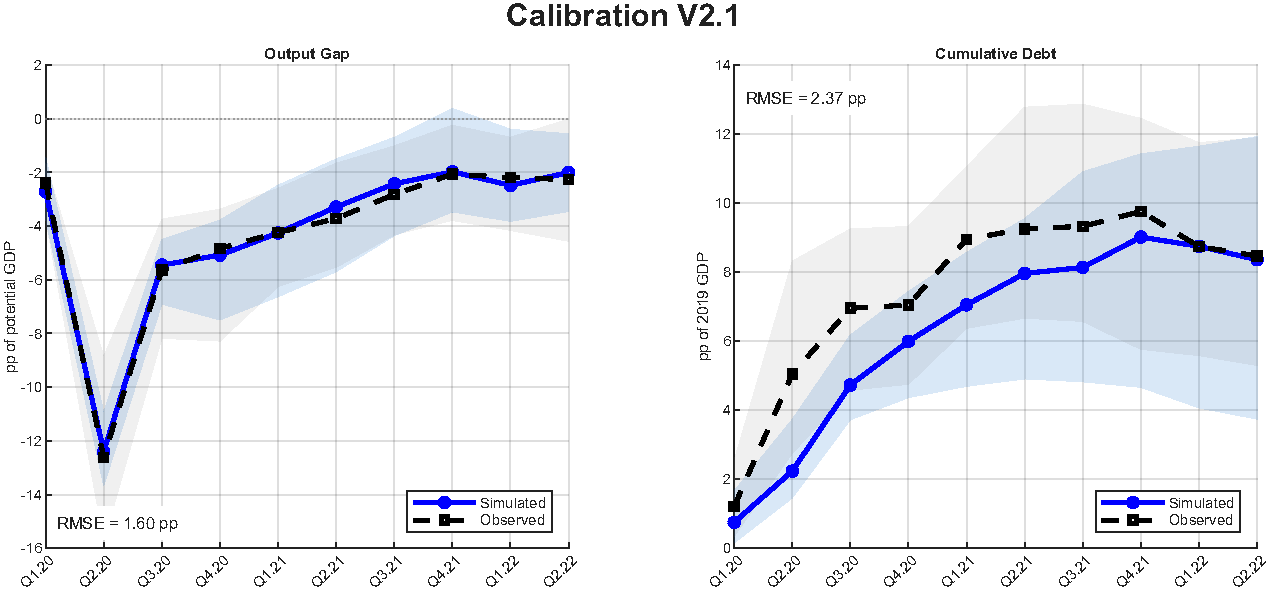
\includegraphics[width=\textwidth]{Validation_cal.pdf}
    \caption{Calibration across OECD Median}
    \label{fig:composition}
\end{figure}



\subsection{Challenges and further Steps}

\subsubsection{Completed Steps}
\begin{itemize}
  \item Literature review, positioning, and formulation of the 
    research question.
  \item Formalization of the pandemic macroeconomic environment, 
    including the distinction between the channels.
  \item Data collection, cleaning, and documentation of the 
    proprietary fiscal micro-database; descriptive analysis 
    and documentation of the codebook.
  \item Model formulation and first calibration via forward roll.
  \item Empirical implementation of the output and debt 
    equations, including identification strategy, 20-specification 
    robustness structure for $\hat{\eta}_p$, and CP decomposition 
    by accounting treatment in the debt equation.
  \item First draft including theoretical framework, literature 
    positioning, contribution, model specification, 
    identification strategy, data description, and preliminary 
    empirical results.
\end{itemize}

\subsubsection{Planned Steps}
\begin{itemize}
  \item Finalize the interpretation of estimated coefficients and test whether the CP decomposition on the output side can be extended to a three-way split (above-the-line, loans, guarantees).
  \item Complete the full robustness checklist (outlier exclusion, 
alternative controls, sample variations, sample splits, 
alternative estimators such as GMM) to address potential 
identification threats, including the composition and 
aggregation of the containment index, cross-country 
heterogeneity, and residual confounders.
  \item Refine the calibration, solve the iLQR optimal control 
    problem, and generate counterfactual trajectories and 
    country-specific Pareto frontiers in output-debt space.
  \item Compute country-level welfare implications and interpret 
    the results relative to the research question.
  \item Write the conclusion and finalize the paper, including 
    appendix, online appendix, and replication package.
\end{itemize}

\subsubsection{Open Questions}
\begin{itemize}
  \item Whether the three-way CP decomposition on the output 
    side remains cleanly identified.
  \item The source of the level offset in the calibrated debt 
    path.
  \item The extent to which iLQR counterfactual trajectories 
    remain within the empirical support of the linearly estimated 
    coefficients, and how to communicate the boundary of valid 
    extrapolation.
  \item How best to frame the paper's main contribution: the 
    empirical identification of the CP persistence channel, the 
    integrated estimation-calibration framework, or the policy 
    implication that contingent instruments dominate in the 
    output-debt trade-off.
\end{itemize}




\newpage
\section{The Wrong Side of Disruption: Did Digital Innovation Reduce Drug Market Frictions?}
\label{sec:paper2}

The ``War on Drugs,'' launched by President Nixon in 1971, seems to be lost. In the United States, drug-related deaths have become the number one cause of death for adults under 45, with over 100,000 fatalities per year, mainly due to deadly opioids. While the opioid crisis is largely concentrated in North America, the consumption of hard drugs is soaring globally. In Europe, cocaine consumption has almost tripled since 2012 according to wastewater analyses \citep{wastewater_2026}; among young adults in Zurich, nearly one in four has consumed cocaine at least once \citep{quednow_uzh_2025}; new psychoactive substances are flooding the market; and consumption continues to rise. This trend extends well beyond Europe: in Africa, overall drug consumption is projected to increase by 40\% by 2026 \citep{africa_2025}, and Southeast Asia is experiencing an unprecedented methamphetamine crisis \citep{asia_2025}. The associated costs are staggering: in the United States alone, healthcare, lost productivity, and crime-related expenses are estimated at around one trillion USD per year --- not counting the value of statistical lives lost, the destabilization of entire nations, or the opportunity costs of mass incarceration \citep{ncdas_2025, whitehouse_opioid_2025}. Yet despite international cooperation among authorities to target the highly concentrated production and supply of drugs --- leading to record seizures every year, increasing global spending on international drug enforcement exceeding 100 billion USD per annum, unprecedented advances in surveillance, information technology, and public awareness --- drug prices have fallen, purity has increased, and consumption has surged \citep{count_costs_2013}. In a report published in 2014, followed by another in 2016, signed by five Nobel laureates in Economics, including Kenneth Arrow and Oliver Williamson, the authors concluded:

\begin{quote}
\textit{``The strategy has failed based on its own terms. Evidence shows 
that drug prices have been declining while purity has been increasing 
[\ldots] despite drastic increases in global enforcement spending. It is 
time to end the `war on drugs' and massively redirect resources towards 
effective evidence-based policies underpinned by rigorous economic 
analysis.''} \citep{lse_2014}
\end{quote}

\noindent The scientific literature strongly supports this conclusion. \citet{pollack_reuter_2014} find little evidence that raising the risk of arrest, incarceration, or seizure at any level of the distribution system raises retail prices, and \citet{caulkins_reuter_taylor_2006} show that cocaine and heroin prices have fallen substantially during a period of massive increases in enforcement. The European data confirm this pattern: the nominal street price of a gram of cocaine has remained roughly stable over the past 15 to 20 years, while purity has increased by 30--45\% since 2013 \citep{euda_europol_cocaine_2022, werb_2011_violence}. Several economic forces explain this failure. Taking cocaine as an illustrative case, the farmgate price of coca accounts for less than one percent of the European street price, so even substantial increases in producer-level risk barely transmit to retail \citep{caulkins_reuter_2010}. Enforcement risk is itself not a marginal shock but a structural feature of the industry: risk premia are already priced into the distribution chain, and incremental increases in enforcement intensity move them only at the margin \citep{becker_murphy_grossman_2006}. At the same time, production and logistics have experienced substantial productivity gains --- coca yields per hectare are increasing \citep{unodc_2024}, synthetic production of methamphetamine and new psychoactive substances has scaled rapidly, and containerised trafficking has lowered transport costs --- shifting the supply curve outward. Enforcement also selects on organisational efficiency, eliminating the weakest operators and leaving a more concentrated and resilient set of suppliers \citep{castillo_mejia_restrepo_2020}. Finally, the spatial substitutability of production --- the ``balloon effect'' --- means that disruption in one region is offset by expansion in another, rendering the global supply elasticity close to zero \citep{mejia_restrepo_2016}. Taken together, these forces generate a persistent condition of excess supply at low and stable prices, in which the binding constraint on aggregate consumption is not the seller's willingness to supply but the buyer's cost of participating in the market.

This buyer-side constraint is itself shaped by the structure of demand. Demand for addictive drugs is inherently inelastic.\footnote{A meta-analysis by \citet{gallet_2014} places the elasticity at roughly $-0.5$ to $-0.8$.} Pivoting the demand curve is therefore structurally difficult. Shifting it horizontally, by contrast, is not subject to the same constraint, and the scope for such shifts depends on who the marginal consumer is and on which margin the response operates. In opioid markets, dependent users dominate and consumption is largely sustained by addiction; the response operates almost entirely along the intensive margin, and demand shifts there have been driven primarily by the increasing potency of the substances themselves, from prescription opioids to heroin to fentanyl. For other hard drugs such as cocaine, MDMA, ketamine or amphetamine, a substantial share of consumption is recreational and discretionary, at least at the initiation stage, and aggregate demand can shift along both the extensive and the intensive margin. \citet{galenianos_2012} argue that in retail drug markets the relevant price a buyer faces is a vector comprising the monetary price, search costs (the time and effort required to locate a willing seller), quality uncertainty and moral hazard (purity is not observable before purchase), arrest and health risks, and social stigma. This framework is key to interpreting the European data. A pure supply expansion would move quantities along a fixed demand curve and lower the monetary price; a pure demand expansion would move quantities along a fixed supply curve and raise the monetary price. Given excess supply and stable monetary prices, this shift plausibly originates in the non-monetary components of the effective price of demand. In a follow-up paper, \citet{galenianos_2017} structurally estimate the model on US crack cocaine data and find that eliminating moral hazard alone would raise average purity by 20\%, reduce purity dispersion by 80\%, increase the number of active buyers by 7\%, and raise aggregate consumption by approximately 12\%.\footnote{See \citet{galenianos_2017}, Table 4, and \citet{galenianos_2012}, Proposition 7.} This pattern --- higher purity, more active buyers, rising consumption at stable monetary prices --- is precisely what the European data display, raising the question of whether a broader reduction in the price vector is driving the observed surge in consumption.

Analyzing the structure of the illicit drug market over the last fifteen years, it becomes clear that it has changed fundamentally. As Boris Quednow, a leading addiction researcher at the University of Zurich, summarized: \textit{``In the past, people had to seek out shady dealers; today, drugs can be ordered contact-free via social media or messenger services and delivered within minutes.''} \citep{quednow_uzh_2025}. While darknet markets first demonstrated that drugs could be traded online, the market has since evolved well beyond the dark web. On Snapchat, Instagram, and other social media platforms, dealers advertise openly using coded emojis and hashtags --- operating with high efficiency, supported by platform algorithms that actively recommend new dealer profiles to users \citep{demant_emcdda_2023}.\footnote{In a netnographic study commissioned by the EMCDDA, a newly created user profile identified and connected with multiple active cocaine dealers within a single day, and was offered a position as a delivery driver within a week \citep{demant_emcdda_2023}.} Encrypted messaging apps like Telegram host dedicated drug-selling groups with administrator-enforced rules, review systems, and automated bots --- organizational structures that closely resemble legitimate e-commerce \citep{dewey_2024_telegram}. Payment is made in cash or cryptocurrency, and the drugs are delivered directly to the buyer by courier, taxi, or food delivery driver --- often within minutes \citep{moyle_2019_drugsforsale}.

Each of these elements reduces a distinct component of the buyer's total cost of consumption. Social media and messaging apps dramatically lower search costs by enabling buyers to identify and contact sellers anonymously within hours. At the same time, online reputation systems, vendor ratings, and escrow services mitigate the moral hazard problem that \citet{galenianos_2017} identify as the second dominant friction in retail drug markets, making product quality partially observable before purchase.\footnote{\citet{bhaskar_2019} show that on darknet platforms, these mechanisms reduce quality dispersion below street-market levels.} Crucially, all of these channels mainly operate through smartphones and none existed in their current form before the rollout of mobile internet across Europe between 2011 and 2018.\footnote{The iPhone was introduced in 2008, WhatsApp in 2009, Instagram in 2010, Snapchat in 2011, Telegram in 2013, and the first major darknet market (Silk Road) operated from 2011 to 2013.}

The diffusion of mobile internet across Europe over the past decade, the corresponding rise of the platforms described above, the theoretical framework linking search frictions to consumption, and the observed surge in drug use together provide a unique opportunity to study what drives the demand for illicit drugs. Europe is particularly well suited for this analysis: unlike the United States, its drug market is not confounded by the fentanyl crisis, and the SCORE wastewater network provides objective, population-level consumption measures \citep{wastewater_2026}. Using this data from up to 168 European cities with varying year coverage, Figure~\ref{fig:binscatter} plots cocaine loads against internet penetration, revealing a clear positive within-city relationship.


\begin{figure}[H]
    \centering
    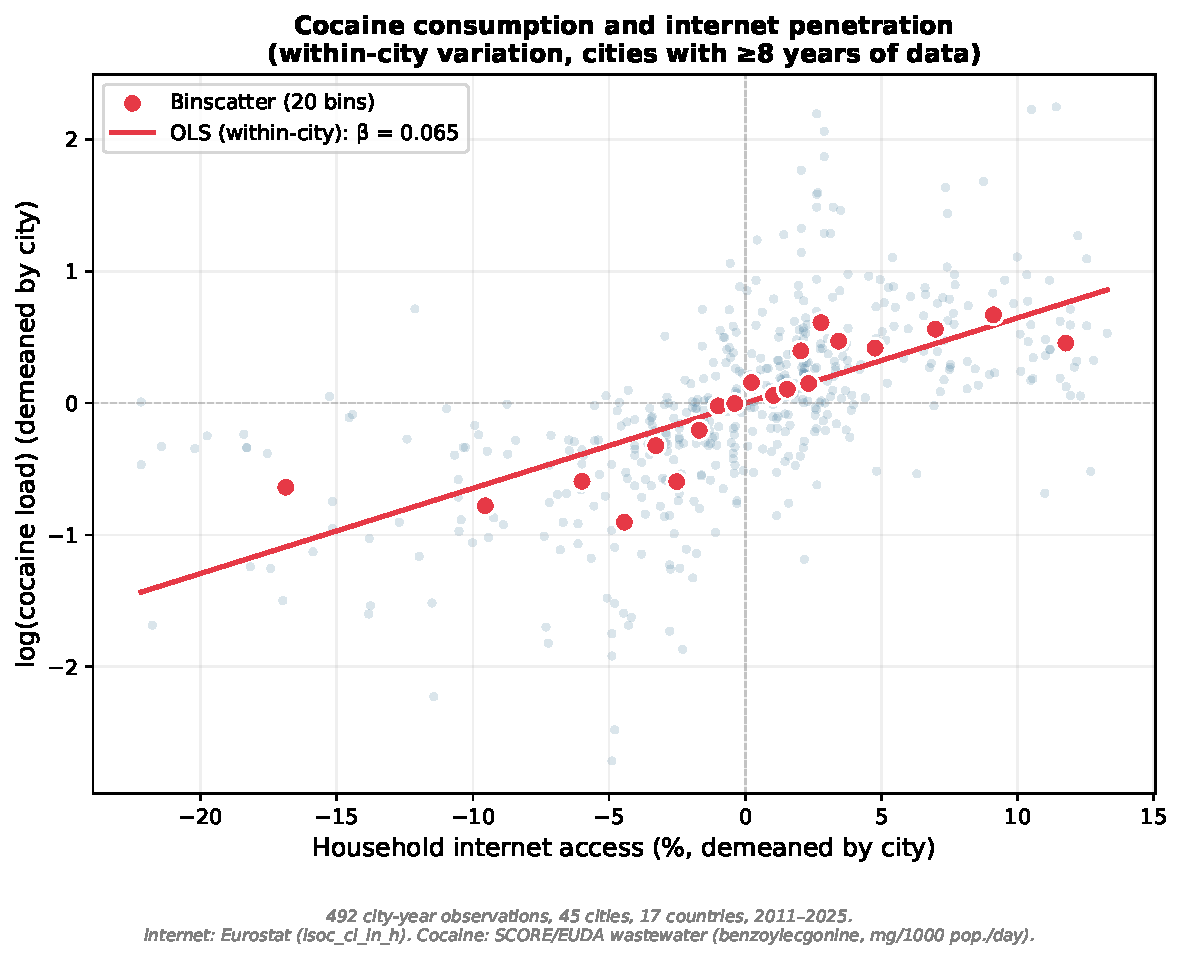
\includegraphics[width=0.55\textwidth]{fig_binscatter_final.pdf}
    \captionsetup{font=scriptsize}
    \caption{Within-city correlation between internet penetration 
    and cocaine consumption. Both variables are demeaned by city. 
    Red dots show a binscatter with 20 equal-sized bins. The 
    sample includes 45 European cities with at least 10 years of 
    observations. Internet access: Eurostat, percentage of 
    households. Cocaine: SCORE/EUDA wastewater data.}
    \label{fig:binscatter}
\end{figure}

\newpage

\noindent As this is a clear naive correlation --- potentially confounded by tourism, urbanisation, income, and other city-level characteristics --- I propose a combined identification strategy that generates exogenous variation in access to mobile internet and platform adoption, and directly tests the mechanism. The main design exploits the European ``Digital Dividend'': the reallocation of UHF spectrum from analog terrestrial television to mobile broadband.\footnote{See alternative possible strategies and further information in Table \ref{tab:internet_proxies}} Two dividends are relevant. The first (800\,MHz) was phased in between 2006 and 2013, with national switch-off dates varying for administrative reasons (Luxembourg 2006, Germany 2008--2009, UK 2012, Poland 2013). The second (700\,MHz) followed between 2015 and 2020 (Germany 2015, France 2015, UK 2016, Italy 2018). In both cases the local capacity gain depended mechanically on the pre-existing share of households relying on terrestrial reception versus cable and satellite, yielding city-level variation that is plausibly exogenous to drug demand. A feasibility check on the availability of sub-national pre-treatment terrestrial shares for both windows is a prerequisite and will determine the main specification; the other dividend then serves as robustness. Methodologically, the design can be implemented as a shift-share event study with national switch-off timing interacted with the pre-treatment terrestrial share, or equivalently as an IV for mobile internet penetration using the same interaction as instrument. %City fixed effects absorb time-invariant heterogeneity; country $\times$ year fixed effects absorb global supply shocks. Clustering operates at the city level (168 clusters).

A limitation of the Digital-Dividend design is that it instruments the enabling infrastructure rather than platform use directly. I plan to address this with two complementary strategies. First, a staggered DiD design around city-level food-delivery launches (Uber Eats, Deliveroo, Glovo, Wolt) because \citet{moyle_2019_drugsforsale} show that drug delivery in Europe increasingly uses the same gig-economy infrastructure as food delivery and launch sequences follow business decisions rather than local drug demand. Second, I plan to complement both designs with event studies around sharp disruptions to online drug markets, exploiting high-frequency wastewater data where available.\footnote{Switzerland (EAWAG/DroMedArio): 10 cities with continuous monitoring since 2021, samples every 13 days; United Kingdom (Home Office WWAP): $\sim$50 sites since May 2021; and individual research laboratories in Barcelona, Milan, Antwerp, and Oslo with varying coverage.} Candidate events include the arrest of Telegram founder Pavel Durov in August 2024, which temporarily disrupted trust in encrypted drug-selling channels, and the COVID-19 lockdowns, which eliminated street-level dealing while leaving digital channels intact. If consumption drops sharply when a major platform is disrupted but recovers as users migrate to alternatives, this constitutes direct evidence for the platform mechanism. 

While a growing body of research has documented the emergence of new forms of online drug trade, to the best of my knowledge no study has yet provided causal evidence linking technology-driven reductions in market frictions to the observed increase in consumption. The theoretical framework suggests that this link is likely, and establishing it empirically would constitute a substantial contribution to the literature --- one that could help redirect the ``war on drugs'' away from its failed supply-side focus toward the evidence-based, demand-centred policies that \citet{lse_2014} and the Nobel laureates who signed their report have long called for.


\medskip
\noindent \textit{Remark: The SCORE panel is unbalanced and based on single-week annual campaigns; a data-quality audit is a prerequisite. The Digital-Dividend design depends on the availability of sub-national pre-treatment terrestrial shares, which determines the feasibility of the main specification (see Table~\ref{tab:internet_proxies} and Table~\ref{tab:identification_strategies} for alternative strategies).}


\newpage
\bibliographystyle{plainnat}
\bibliography{references}

\newpage

%\noindent A good starting point may be to listen to those who drive the supply side of this global epidemic. As Joaqu\'{i}n ``El Chapo'' Guzm\'{a}n, once the world's most powerful drug trafficker, put it: \textit{``If there was no consumption, there would be no 
%sales.''}\footnote{When asked about his responsibility for global drug consumption, Guzm\'{a}n responded: \textit{``If there was no consumption, there would be no sales. It is true that consumption, day after day, becomes bigger and bigger. So it sells and sells.''} 
%See \citet{penn_elchapo_2016}.}

\section*{Appendix}

\subsection{Identification Discussion}
\begin{table}[H]
\centering
\footnotesize
\caption{Measures and proxies for mobile internet penetration}
\label{tab:internet_proxies}
\begin{tabular}{p{3.8cm} p{2.8cm} p{1.8cm} p{1.4cm} p{1.8cm} p{1.8cm}}
\hline\hline
\textbf{Proxy} & \textbf{Source} & \textbf{Granularity} & \textbf{Period} & \textbf{DiD/ES} & \textbf{IV} \\
\hline
\multicolumn{6}{l}{\textit{Panel A: Outcome / penetration measures}} \\[3pt]

Households with internet access & 
Eurostat \texttt{isoc\_r\_iuse\_i} & 
NUTS2 & 
2006-- & 
High & 
Low \\[4pt]

Households with broadband & 
Eurostat \texttt{tgs00048} & 
NUTS2 & 
2006-- & 
High & 
Low \\[4pt]

4G coverage (\% population) & 
EU DESI, Omdia, Opensignal & 
Country, partly NUTS2 & 
2012-- & 
Very high & 
Medium \\[4pt]

Mobile broadband subscriptions per capita & 
OECD, ITU & 
Country & 
1990-- & 
Medium & 
Low \\[4pt]

Smartphone penetration & 
Eurostat, GSMA & 
Country, partly NUTS2 & 
2011-- & 
High & 
Low \\[4pt]

Data volume per subscription (GB/month) & 
GSMA Intelligence, Cisco VNI & 
Country & 
2010-- & 
High & 
Low \\[4pt]

Ookla Speedtest (median DL/UL) & 
Ookla Open Data & 
$\sim$600m tile & 
2019-- & 
High (late start) & 
Low \\[6pt]

\hline
\multicolumn{6}{l}{\textit{Panel B: Infrastructure shocks and historical instruments}} \\[3pt]

\textbf{First Digital Dividend (800\,MHz switch-off $\times$ terrestrial share)} & 
ITU, SES Monitor, national regulators & 
Country $\times$ NUTS2 & 
2006--2013 & 
High & 
\textbf{Very high} \\[4pt]

\textbf{Second Digital Dividend (700\,MHz switch-off $\times$ terrestrial share)} & 
ITU, EU Digital Agenda, national regulators & 
Country $\times$ NUTS2 & 
2015--2020 & 
\textbf{Very high} & 
\textbf{Very high} \\[4pt]

4G auction date & 
National regulators & 
Country & 
one-off & 
Very high & 
--- \\[4pt]

4G commercial launch date & 
GSMA, national operators & 
Country, partly city & 
one-off & 
Very high & 
--- \\[4pt]

Number of base stations & 
National regulators, OpenCellID & 
City / NUTS3 & 
variable & 
High & 
Medium \\[4pt]

TRI $\times$ Post-4G & 
NASA SRTM + auction dates & 
City & 
--- & 
--- & 
Low \\[4pt]

PSTN-MDF distance & 
\citet{falck_2014} & 
Municipality (DE only) & 
historical & 
Medium & 
High (DE only) \\[4pt]

Historical copper network density & 
ITU 1990s & 
Country & 
historical & 
Low & 
High \\[4pt]

Historical TV mast locations & 
EBU transmitter registry & 
Geo-point & 
historical & 
Low & 
High \\[6pt]

\hline
\multicolumn{6}{l}{\textit{Panel C: Platform-specific proxies}} \\[3pt]

\textbf{Food-delivery launch date} & 
Press releases & 
City & 
one-off & 
\textbf{Very high} & 
\textbf{Very high} \\[4pt]

Russian-speaking diaspora share & 
Eurostat Census 2011/2021 & 
NUTS3 & 
two waves & 
Low & 
High \\[4pt]

Mobile data price (per GB) & 
Cable.co.uk, ITU & 
Country $\times$ year & 
2011-- & 
High & 
Medium \\[4pt]

Facebook Social Connectedness Index & 
Meta Data for Good & 
NUTS3 & 
2020+ & 
Medium & 
Medium \\[4pt]

E-Government Index & 
EU DESI & 
Country, NUTS2 & 
2014-- & 
Medium & 
Low \\[3pt]

\hline\hline
\end{tabular}
\end{table}


\begin{table}[H]
\centering
\footnotesize
\caption{Comparison of identification strategies}
\label{tab:identification_strategies}
\begin{tabular}{p{4.2cm} p{2.6cm} p{0.9cm} p{1.6cm} p{1.3cm} p{1.8cm}}
\hline\hline
\textbf{Strategy} & \textbf{Exogeneity} & \textbf{Clust.} & \textbf{Within-country var.} & \textbf{Wi-Fi issue} & \textbf{Mechanism} \\
\hline
\multicolumn{6}{l}{\textit{Main designs}} \\[3pt]

\textbf{Digital Dividend (DiD / IV)} & 
High (historical + administrative) & 
168 & 
Yes & 
Partial (mobile LATE) & 
No \\[4pt]

\textbf{Food-delivery launch DiD} & 
High (business decision) & 
168 & 
Yes & 
Resolved & 
\textbf{Yes} \\[6pt]

\hline
\multicolumn{6}{l}{\textit{Robustness and alternatives}} \\[3pt]

Staggered DiD, 4G auction & 
High (country-level) & 
26 & 
No & 
No & 
No \\[4pt]

TRI $\times$ Post-4G & 
Low (urbanisation confounding) & 
168 & 
Yes & 
No & 
No \\[4pt]

City-level 4G rollout DiD & 
Low (operator selection) & 
168 & 
Yes & 
No & 
No \\[4pt]

Czernich copper density & 
High (historical) & 
26 & 
No & 
No & 
No \\[4pt]

PSTN-MDF distance (Falck) & 
High (historical) & 
many (DE only) & 
Yes & 
No & 
No \\[4pt]

Border RD & 
High (border parity) & 
city-pairs & 
Yes & 
No & 
No \\[4pt]

Russian diaspora $\times$ Telegram & 
High (historical migration) & 
168 & 
Yes & 
Partial & 
\textbf{Yes} \\[3pt]

\hline\hline
\end{tabular}
\end{table}

\newpage
\subsection{Ideas Event studies}

\begin{enumerate}
    \item \textbf{Telegram/Durov arrest} (August 2024): The arrest of Telegram founder Pavel Durov in France disrupted Telegram-based drug-selling groups across Europe, providing the most recent and arguably cleanest demand-side shock to messenger-based drug markets. Primary candidate for high-frequency wastewater event study.
    
    \item \textbf{COVID-19 lockdowns} (March 2020): Lockdowns simultaneously restricted physical drug markets while leaving digital channels intact. Cities with higher pre-lockdown internet penetration should have experienced smaller declines in consumption, which can be tested as a triple-difference design (city $\times$ time $\times$ lockdown $\times$ internet) on the SCORE annual panel where both 2019 and 2020 are observed.
    
    \item \textbf{Darknet market shutdowns} (e.g., Hydra, April 2022): Law enforcement takedowns abruptly raise search costs for online buyers. If platforms causally reduce transaction costs, consumption should drop after shutdowns and recover as users migrate. Null effects are interpretable: \citet{soska_christin_2015} document that substitution typically occurs within weeks, which would indicate the platform channel is resilient rather than absent.
    
    \item \textbf{EncroChat hack} (June 2020) and \textbf{SkyECC dismantling} (March 2021): European law enforcement operations targeting encrypted communication platforms of organised criminal networks. Primarily affected wholesale and mid-level dealer communication; expected effect on retail consumption operates through upstream supply disruption rather than buyer-facing search frictions. Secondary candidates, included for completeness.
\end{enumerate}


\subsection{Count Fiscal Instruments}
\begin{table}[H]
\centering
\caption{Fiscal Instrument Classification}
\label{tab:fiscal_classification}
\scriptsize
\begin{tabular}{@{}llr@{}}
\toprule
\textbf{Channel} & \textbf{Instruments} & \textbf{Measures} \\
\midrule
\multicolumn{3}{@{}l}{\textit{Capacity Preservation ($F^{CP}$)}} \\[3pt]
\quad Above-the-line
  & Short-time work, payroll subsidies, direct grants
  & 948 \\[3pt]
\quad Below-the-line
  & Government loans, credit guarantees
  & 400 \\[6pt]
\multicolumn{3}{@{}l}{\textit{Demand Injection ($F^{DI}$)}} \\[3pt]
\quad Transfers
  & Cash transfers, unemployment top-ups, ad-hoc benefits
  & 346 \\[3pt]
\quad Tax measures
  & Income tax relief, VAT reductions, tax credits
  & 162 \\[3pt]
\quad Demand stimulus
  & Infrastructure, green investment, tourism support
  & 38 \\[6pt]
\multicolumn{3}{@{}l}{\textit{Health ($F^{H}$)}} \\[3pt]
\quad
  & Medical procurement, hospital capacity, vaccine rollout
  & 232 \\[6pt]
\midrule
\multicolumn{2}{@{}l}{\textit{Excluded: Tax deferrals (IMF Cat.\ 3)}}
  & 154 \\[3pt]
\multicolumn{2}{@{}l}{\textit{Excluded: Unclassified and excluded policy codes}}
  & 21 \\[3pt]
\midrule
\multicolumn{2}{@{}l}{\textbf{Total}}
  & \textbf{2,301} \\
\bottomrule
\end{tabular}

\smallskip
\end{table}


\end{document}



